% 本工作流输出 Word（.docx），图表由 paper/main.md 以 Markdown 语法引用 figures/*.png 与
% figures/TABLE_*.md。此文件仅作为 paper-figure 步骤完成标记与图表清单，供下游参考。
%
% ===== 数据图（11 张，均为 350 DPI PNG）=====
% fig_eda_style_pca.png        数据探索：22 风格样本量 + 化学谱 PCA 按风格分离（2 panel）
% fig_q1_missing_pattern.png   问题一：缺失模式矩阵 + 列缺失率条形
% fig_q1_pred_perf.png         问题一：50 感官维交叉验证 QWK 排序（棒棒糖，双列）
% fig_q1_calibration.png       问题一：代表维连续校准散点 + 等级混淆热力（2 panel）
% fig_q2_coexpr_network.png    问题二：化合物共表达网络（社区着色、度定大小）
% fig_q2_top3_heatmap.png      问题二：12 维 × 15 关键化合物 Top-3 融合权重热力
% fig_q2_stability.png         问题二：50 维 Top-1 入选频率(Wilson CI) + 跨方法 Jaccard
% fig_q2_chem_sensory_corr.png 问题二：化学 × 感官交叉相关矩阵（合理性证据）
% fig_q3_style_radar.png       问题三：Tripel/Kriek/Lambic 生成谱感官画像雷达
% fig_q3_realvsgen.png         问题三：真实 vs 生成化学谱 PCA 重叠（2 panel）
% fig_q3_transfer_defect.png   问题三：跨风格迁移 4 缺陷化合物哑铃图（阈值合规）
%
% ===== 结果表（5 张，Markdown 三线表）=====
% TABLE_q1_model_cmp.md  Q1 主模型 vs 基线整体对比
% TABLE_q1_perf.md       T1 代表性感官维预测性能 QWK/MAE/R2
% TABLE_q2_top3.md       T2 感官维 Top-3 关键化合物 + 稳定性
% TABLE_q3_style.md      T3 三代表风格生成质量概览
% TABLE_q3_defect.md     T3 跨风格迁移缺陷阈值合规
%
% ===== HTML 流程/架构图（paper-figure-html 产出，mono 纯黑白；Word 模式转 350 DPI PNG）=====
% fig_roadmap   整体技术路线图（三问递进：数据基础→Q1 预测→Q2 归因→Q3 生成迁移→综合输出）
% fig_arch_q1   问题一感官评分 pipeline 架构（缺失感知梯度提升→多输出有序回归→0-6 分箱→分层交叉验证）
% fig_arch_q3   问题三风格条件生成 CVAE 架构（编码器→隐空间→条件解码器→缺陷阈值投影→生成谱）
\begin{figure}[H]
\centering
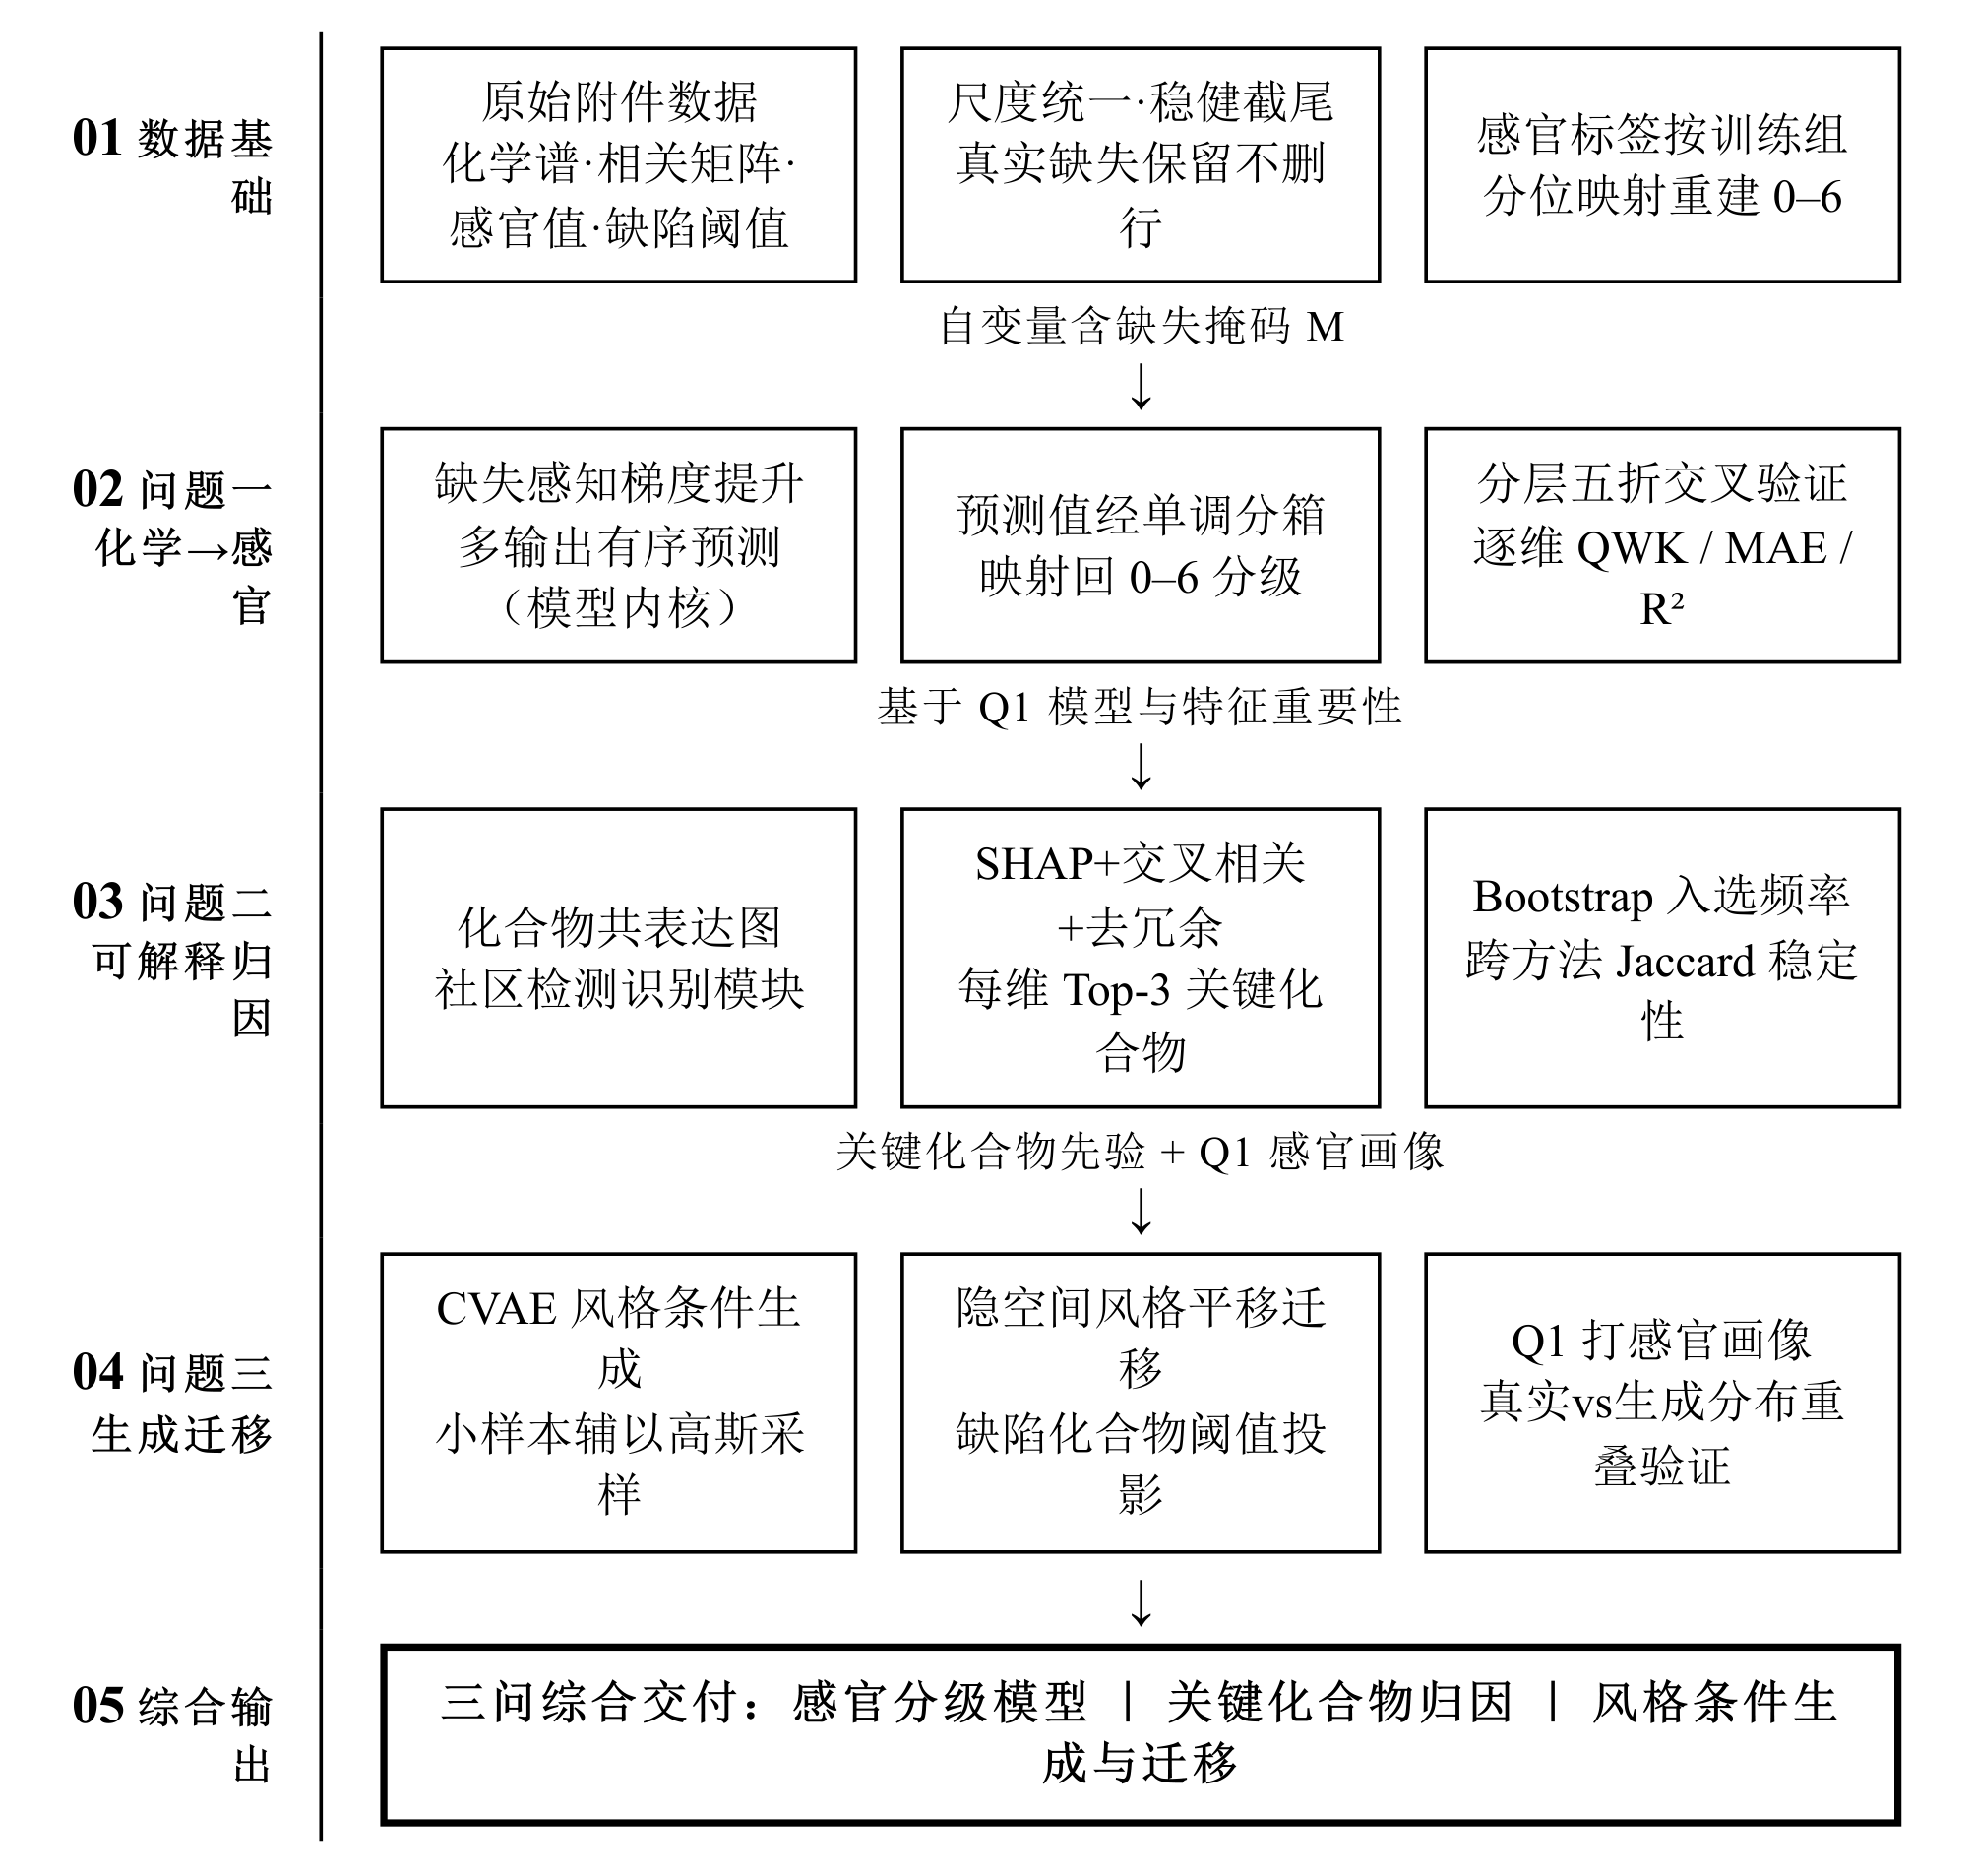
\includegraphics[width=0.90\textwidth,height=0.8\textheight,keepaspectratio]{figures/fig_roadmap.png}
\caption{整体技术路线图}\label{fig:roadmap}
\end{figure}

\begin{figure}[H]
\centering
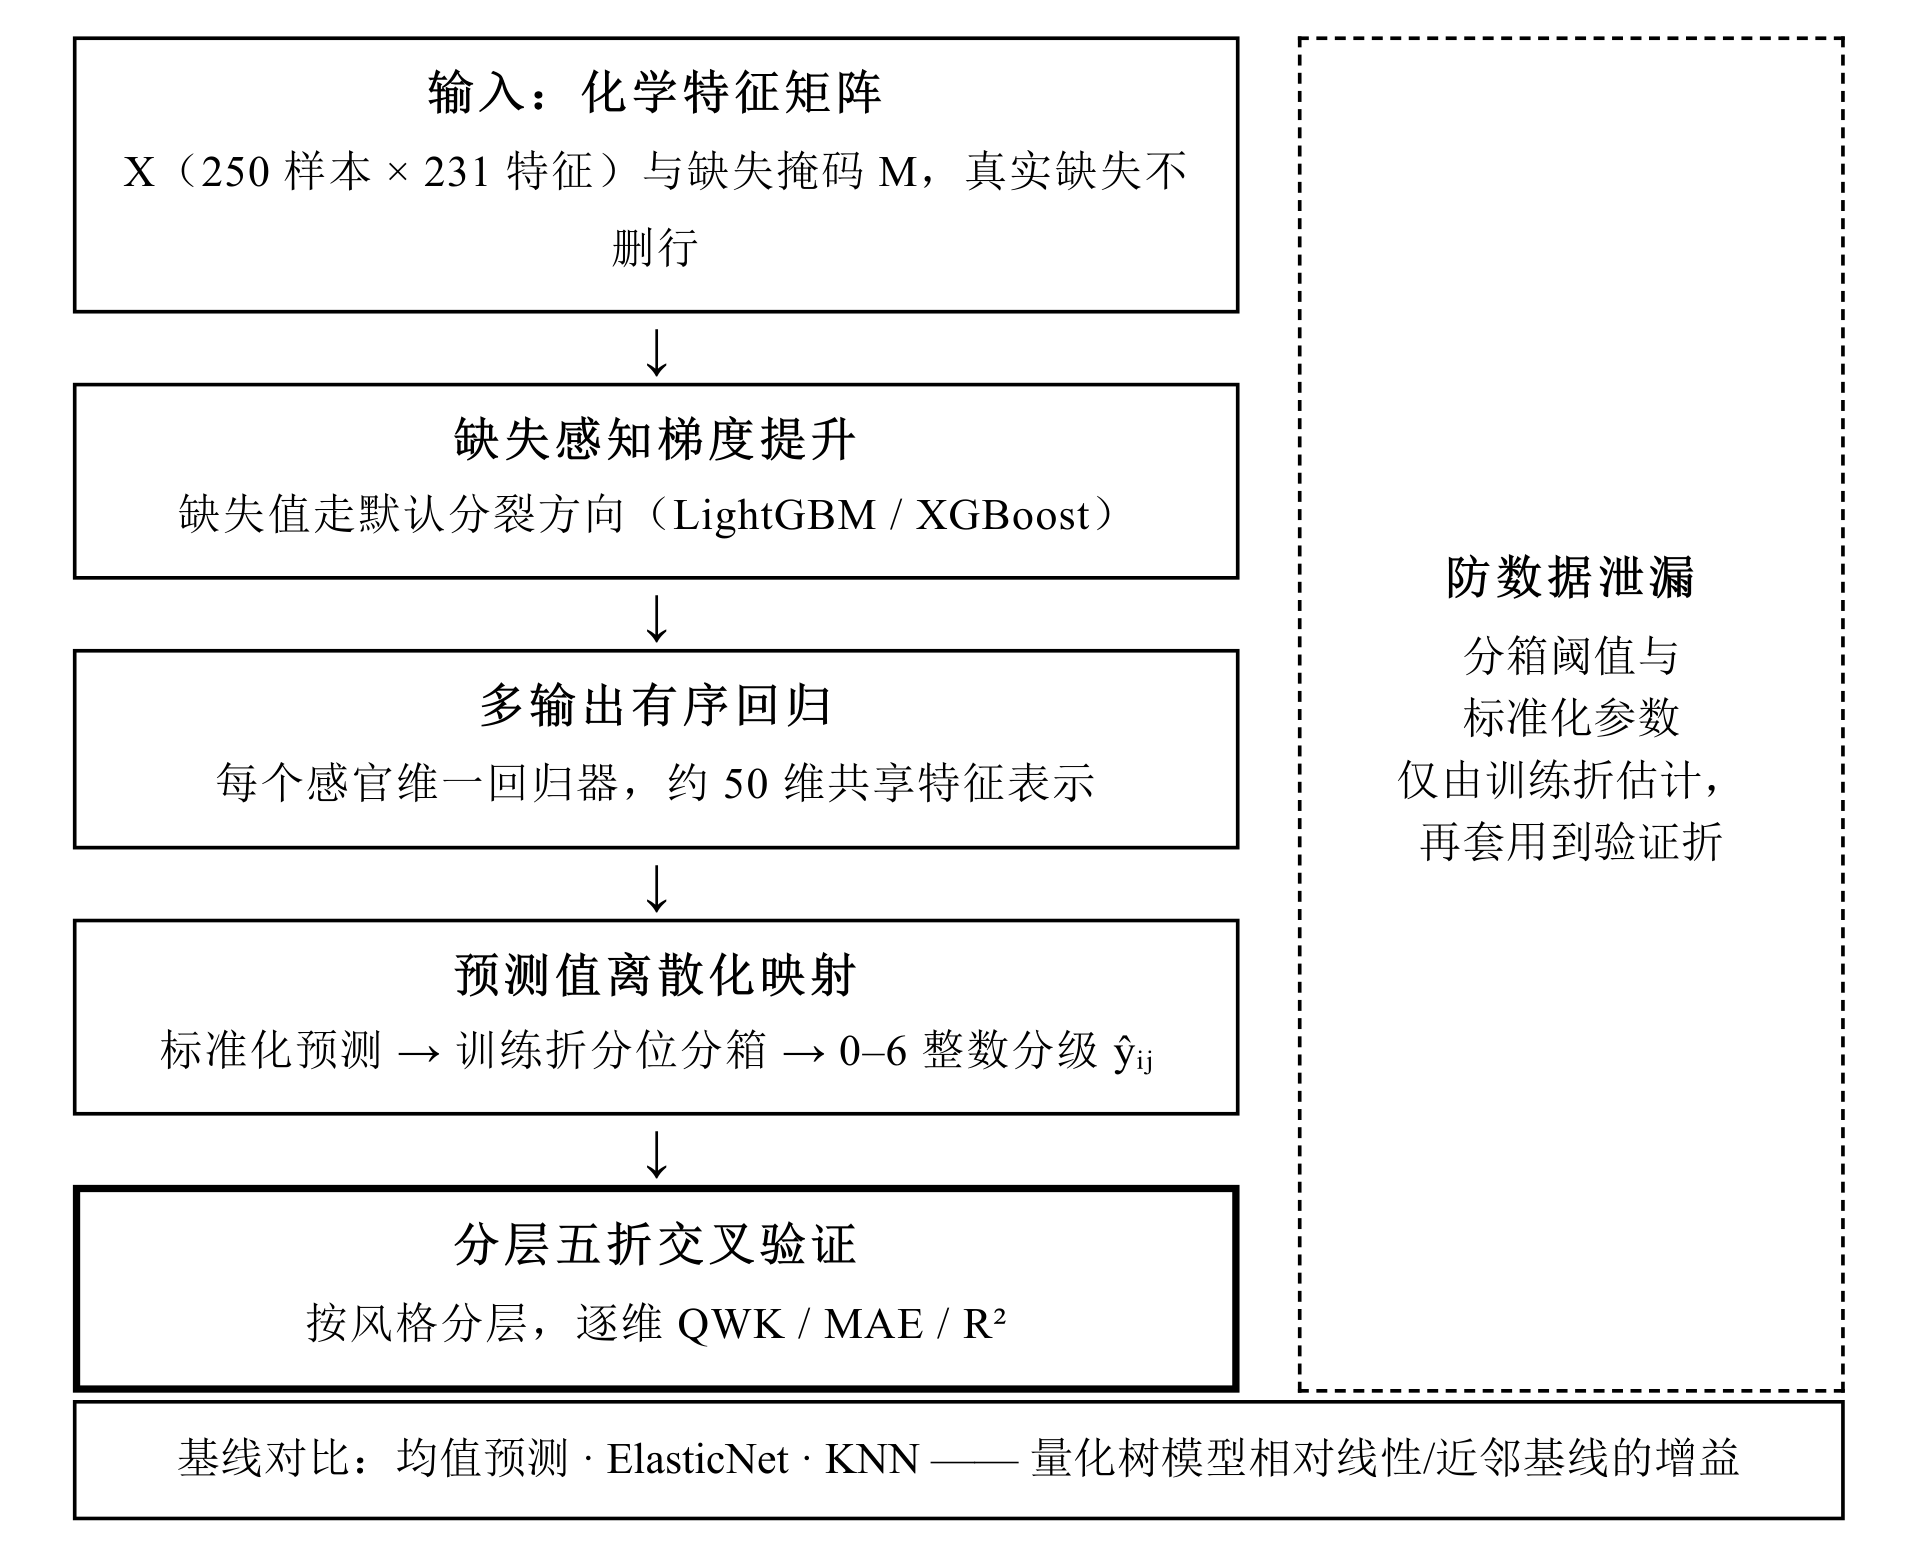
\includegraphics[width=0.78\textwidth,height=0.8\textheight,keepaspectratio]{figures/fig_arch_q1.png}
\caption{问题一感官评分 pipeline 架构}\label{fig:arch_q1}
\end{figure}

\begin{figure}[H]
\centering
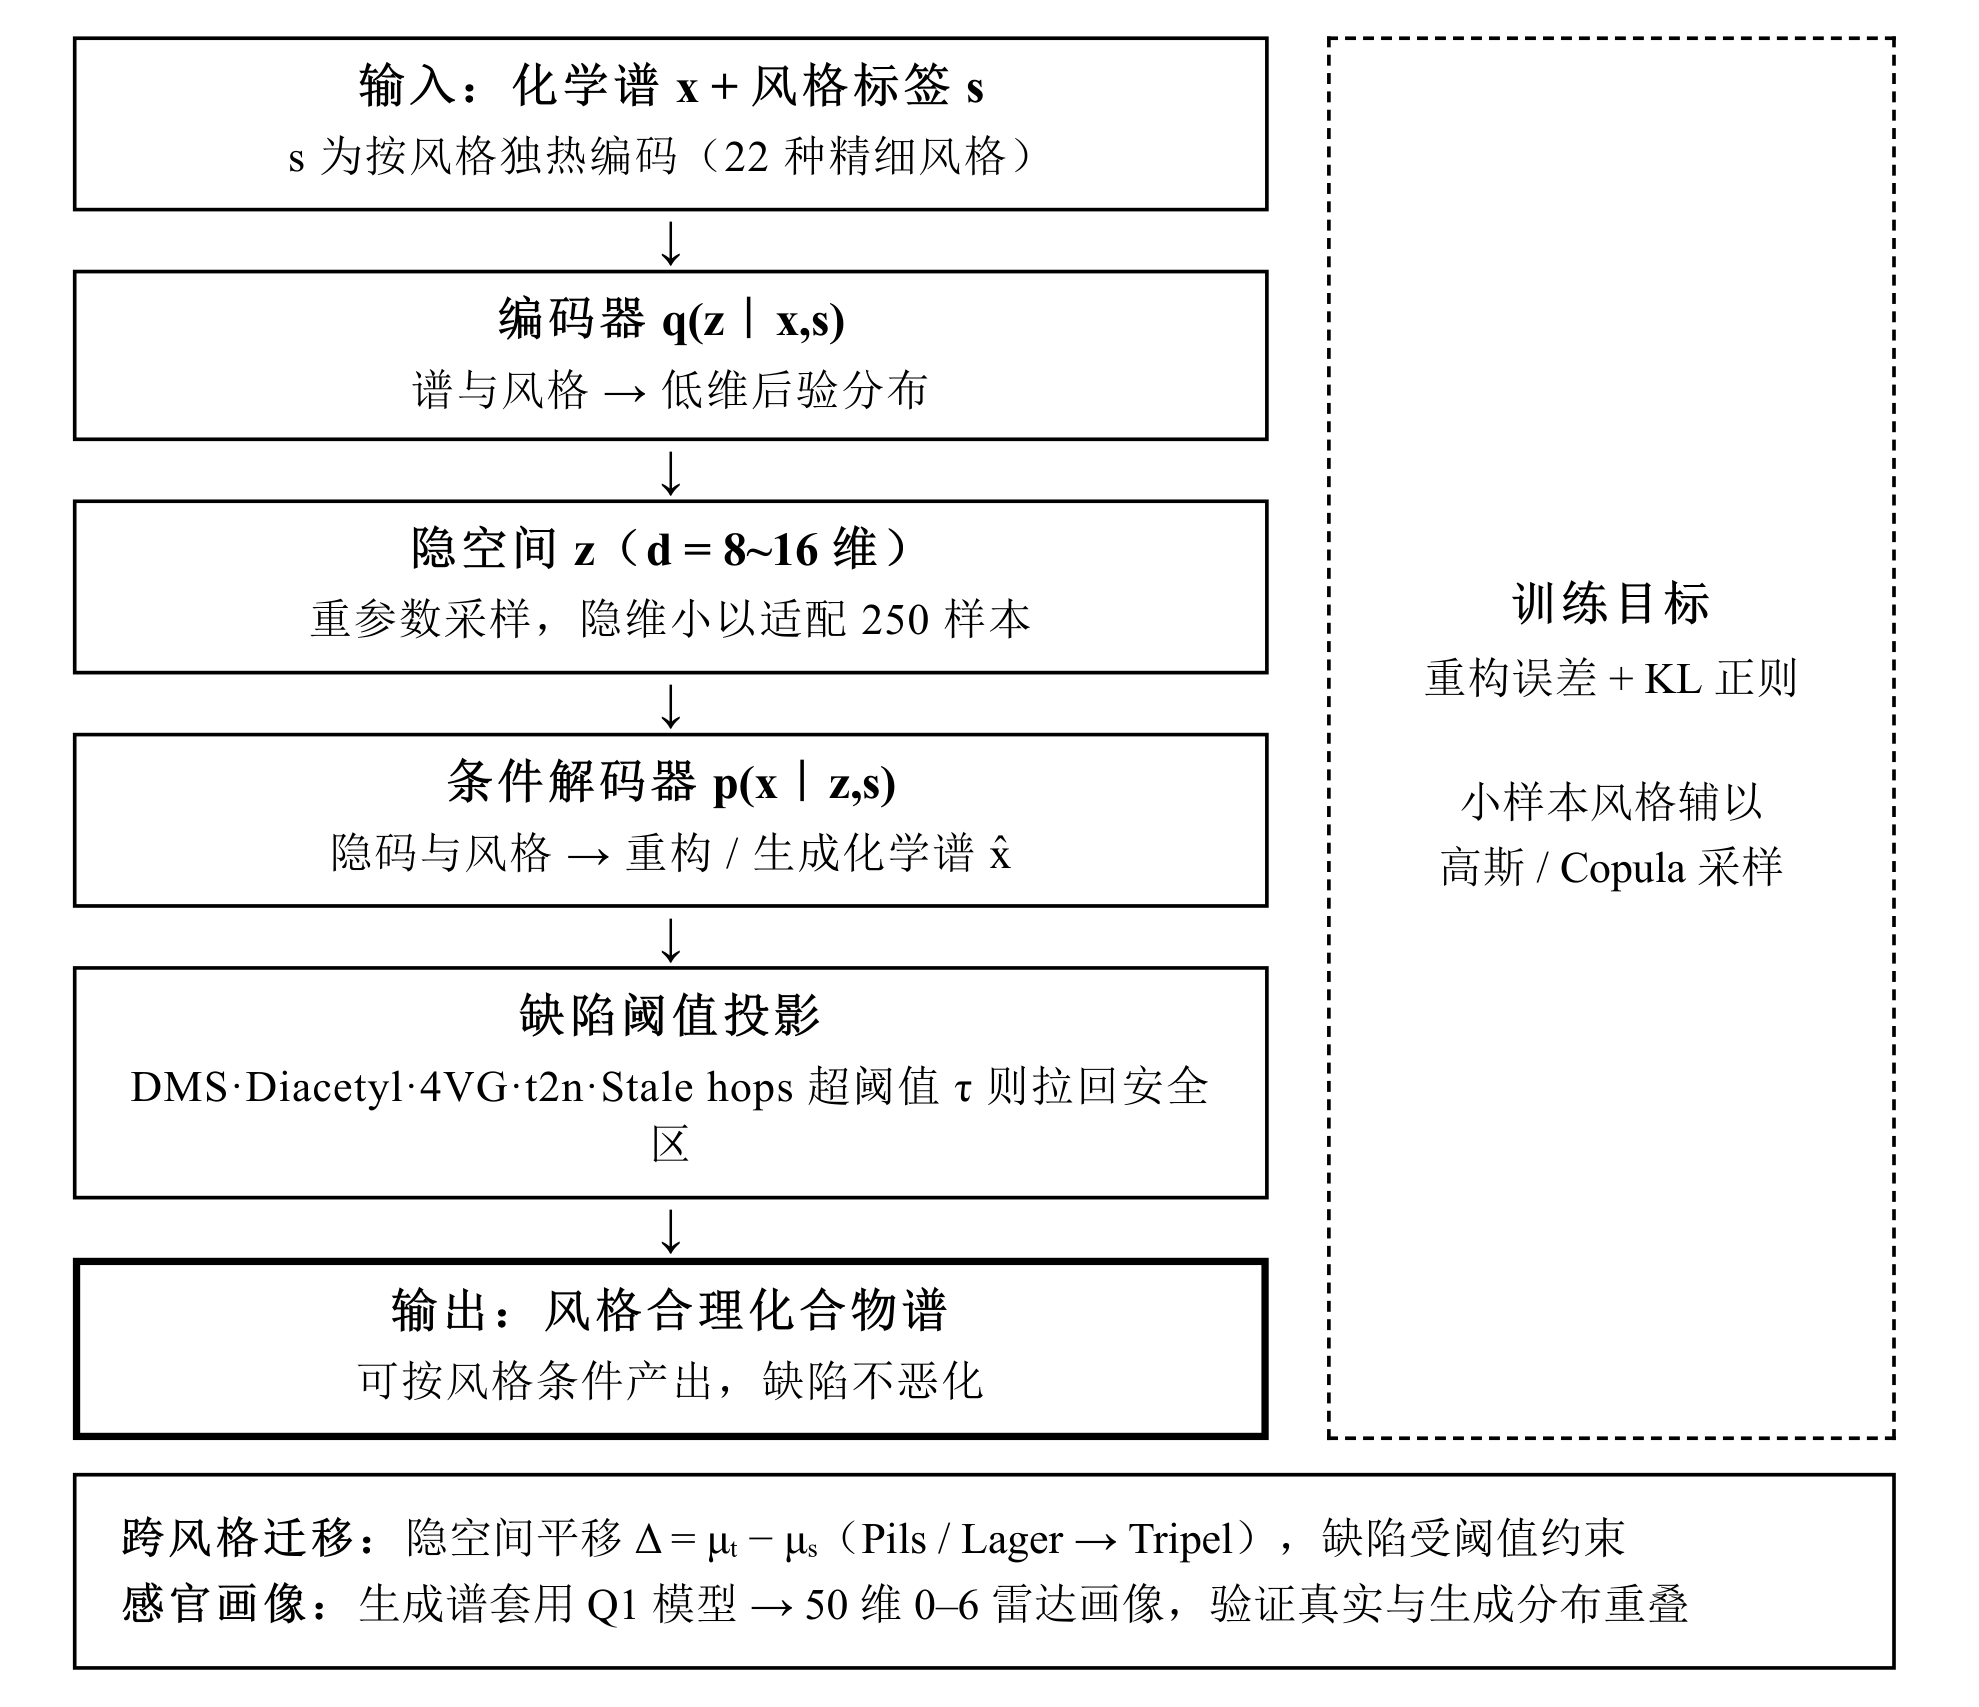
\includegraphics[width=0.82\textwidth,height=0.8\textheight,keepaspectratio]{figures/fig_arch_q3.png}
\caption{问题三风格条件生成（CVAE）架构}\label{fig:arch_q3}
\end{figure}
